% !TEX encoding = UTF-8 Unicode
\documentclass{beamer}

\usepackage{color}
\usepackage{url}
\usepackage[utf8]{inputenc}
\usepackage{graphicx}
\usepackage[english,serbian]{babel}
%\usetheme{Pittsburgh}
%\usecolortheme{beetle}
\setbeamertemplate{navigation symbols}{}

\usepackage{listings}
\definecolor{codegreen}{rgb}{0,0.6,0}
\definecolor{codegray}{rgb}{0.5,0.5,0.5}
\definecolor{codeblue}{rgb}{0.0,0,0.82}
\lstdefinestyle{mystyle}{
    commentstyle=\color{codegreen},
    keywordstyle=\color{codeblue},
    numberstyle=\tiny\color{codeblue},
    stringstyle=\color{codegreen},
    basicstyle=\ttfamily\footnotesize,
    breakatwhitespace=false,
    breaklines=true,
    captionpos=b,
    keepspaces=true,
    showspaces=false,
    showstringspaces=false,
    showtabs=false,
    tabsize=4,
    xleftmargin=3em,
    framexleftmargin=1.5em
}
\lstset{style=mystyle}


\usepackage[font=scriptsize,labelfont=bf]{caption}

\title{Sinteza programa}

\author{ \href{mailto:anja.ivanisevic95@gmail.com}{Anja Ivanišević}\\ \href{mailto:mi14031@matf.bg.ac.rs}{Ivan Ristović}\\ \href{mailto:mi14042@matf.bg.ac.rs}{Milana Kovačević}\\ \href{mailto:vesna.katanic@gmail.com}{Vesna Katanić}}
\date{maj 2018.}


\begin{document}
\begin{frame}
    \titlepage
\end{frame}

\begin{frame}{Uvod}
    TODO
    \begin{itemize}
        \item Automatska sinteza programa ima potencijal da promeni generalni pristup implementaciji programa
        \item Omogućavanje i manje stručnim licima da programiraju
        \item Korisnici daju opis željenih funkcionalnosti programu za automatsko generisanje koda
        \item \emph{Sintezer}) automatski generiše neophodnu implementaciju
    \end{itemize}
\end{frame}

\begin{frame}{Primene}
    \emph{Programiranje vođeno primerima} (eng. \emph{Programming Based on Examples)}:
    \begin{itemize}
        \item Zadaje se šablon koda ili nekoliko primera izlaza programa
        \item Kod se generiše automatski
        \item TODO primer
    \end{itemize}
\end{frame}

\begin{frame}{Primene}
    Neke od oblasti primene sinteze programa koje će biti pokrivene u ovom radu su:
    \begin{itemize}
        \item Priprema podataka
        \item Popravka koda
        \item Sugestije prilikom kodiranja
        \item Grafika
        \item Superoptimizacija
        \item Konkurentno programiranje
    \end{itemize}
\end{frame}

\begin{frame}{Primene - Priprema podataka}
    \begin{itemize}
        \item Proces pripreme često obuhvata sledeće operacije nad podacima:
            \begin{itemize}
                \item izvlačenje
                \item transformacija
                \item formatiranje
            \end{itemize}
        \item Manipulisanje niskama ili izmene samih tipova podataka
        \item Korisnici se zamaraju pisanjem skriptova ili makroa
        \item PBE je idealan za ovakav posao
    \end{itemize}
\end{frame}

\begin{frame}{Primene - Popravka koda}
    \begin{itemize}
        \item Računanje modifikacija programa $P$ koje stvaraju nov program $P'$ takav da zadovoljava specifikaciju $\phi$
        \item Ubacuju se alternativni izbori za izraze u programu
        \item Tehnikama programske sinteze izraza pronađu izrazi koji program dovode u oblik koji zadovoljava $\phi$
    \end{itemize}
\end{frame}

\begin{frame}[fragile]{Primene - Popravka koda - Primer}
    \begin{figure}[!h]
        \centering
        \tiny
        \begin{tabular}{ccc|cc}
            \multicolumn{3}{c|}{Ulaz} & \multicolumn{2}{c}{Izlaz}\\
            inb & usep & dsep & expected & actual \\
            \hline
            1 & 0 & 100 & 0 & 0 \\
            1 & 11 & 110 & 1 & 0 \\
            0 & 100 & 50 & 1 & 1 \\
            1 & -20 & 60 & 1 & 0 \\
            0 & 0 & 10 & 0 & 0 \\
        \end{tabular}

        \centering
        \begin{lstlisting}[language=C, basicstyle=\tiny]
            int buggy(int inb, int usep, int dsep)
            {
                int bias;
                if (inb)
                    bias = dsep; //fix: bias = usep+100
                else
                    bias = usep;
                if (bias > dsep)
                    return 1;
                else
                    return 0;
            }
        \end{lstlisting}

        \caption{Primer koda sinteziranog od strane programa \emph{SemFix} koristeći skup ulaznih i izlaznih test primera.}
        \label{fig:CodeRepair}
    \end{figure}
\end{frame}

\begin{frame}{Primene - Sugestije prilikom kodiranja}
    \begin{itemize}
        \item Podrške okruženja za rad:
        \begin{itemize}
            \item \emph{IntelliSense} za \emph{MS Visual Studio}
            \item \emph{Content Assist} za \emph{Eclipse}
        \end{itemize}
        \item Tehnike za generisanje čitavih jedinica koda:
        \begin{itemize}
            \item \emph{statistički modeli}
            \item \emph{dopuna usmerena tipovima} (eng. \emph{type-directed completion})
            \item ostale tehnike (koriste ih \emph{InSynth} i \emph{Bing Developer Assistant})
        \end{itemize}
    \end{itemize}
\end{frame}

\begin{frame}{Primene - Grafika}
    \begin{itemize}
        \item Konstrukcija ponovljenih objekata
        \item Korišćenjem PBE, korisnik prikaže par primera a sintezer predviđa naredne objekte u nizu
        \item Interaktivno postavljanje grafičkih objekata preko grafičkog interfejsa
        \item Efikasnija geometrijska izračunavanja, brže animacije
    \end{itemize}
\end{frame}


\begin{frame}{Primene - Superoptimizacija}
    \begin{itemize}
        \item Kreiranje optimalnog poretka instrukcija mašinskog koda zarad dobijanja na performansama
        \item Primer
        \begin{figure}[!h]
            \centering
            \small
            \begin{tabular}{rl}
                originalni kod: & $\mathit{prosek}=\frac{x+y}{2}$\\
                optimizovani kod: & prosek = $(x \mid y)-((x \oplus y) \gg 1)$
            \end{tabular}
        \end{figure}
        \item Jedan od načina da se kod automatski optimizuje je korišćenje  \emph{enumerativne pretrage}
    \end{itemize}
\end{frame}

\begin{frame}{Primene - Konkurentno programiranje}
    \begin{itemize}
        \item Pomoć pri pisanju bezbednog kompleksnog višenitnog koda
        \item \emph{Sinteza vođena apstrakcijom}:
        \begin{itemize}
            \item Pravi se apstraktna reprezentacija programa u apstraktnom domenu
            \item Proverava se da li postoji kršenje postavljene specifikacije programa (obično trka za podacima)
            \item Ukoliko postoji prekršenje, menjamo ili apstrakciju (npr. sužavanjem domena) ili sam program dodajući sinhronizacione konstrukte
            \item Ovaj postupak se ponavlja sve dok se ne nađe program koji može biti verifikovan apstrakcijom
        \end{itemize}
    \end{itemize}
\end{frame}

\begin{frame}{Izazovi}
    \begin{itemize}
        \item Sa visokog nivoa, problem sinteze se može razložiti na dva potproblema:
            \begin{itemize}
                \item Definisanje specifikacija željenog programa
                \item Pretraživanje prostora mogućih programa u potrazi za onim koji zadovoljava definisane specifikacije
            \end{itemize}
        \item Prostor programa se povećava eksponencijalno brzo u odnosu na veličinu željenog programa
    \end{itemize}
\end{frame}


\begin{frame}{Izazovi - Definisanje specifikacija}
    \begin{itemize}
        \item Većina programa koji se danas koriste su previše komplikovani da bi se u potpunosti opisali bilo formalnim bilo neformalnim metodama
        \item Potrebno je omogućiti korisniku da definiše željeni program do neke tačke, a da kasnije tokom sinteze, interaktivno sa računarom, postepeno dolazi do rešenja
        \item \emph{FlashFill}
    \end{itemize}
\end{frame}

\begin{frame}{Izazovi - Pretraživanje prostora programa}
    \begin{itemize}
        \item Prostor programa - skup koji sadrži sve moguće programe koji se mogu napisati
        \item Pretraga ovog skupa znači nalaženje programa koji zadovoljava specifikacije
        \item Tehnike pretrage se mogu zasnivati na:
            \begin{itemize}
                \item Enumerativnoj pretrazi
                \item Dedukciji
                \item Tehnikama sa ograničenjima
                \item Induktivnim i statističkim metodama
            \end{itemize}
    \end{itemize}
\end{frame}

\begin{frame}{Izazovi - Pretraživanje prostora programa - Enumerativna pretraga}
    \begin{itemize}
        \item Jedna od najefikasnijih tehnika za generisanje malih programa
        \item Tehnike \emph{čišćenja}
        \item Prvo se na neki način opiše prostor pretrage u kome se nalazi željeni program
        \item Kada se mogući programi numerišu po osobinama, mogu da se odmah odbace oni koji ne zadovoljavaju specifikaciju
        \item Enumerativna tehnika je poluodlučiva
    \end{itemize}
\end{frame}

\begin{frame}{Izazovi - Pretraživanje prostora programa - Deduktivna pretraga}
    \begin{itemize}
        \item Pretpostavka da postoji celokupna formalna specifikacija željenog programa
        \item Rešenje se sintetiše postupkom dokazivanja teorema, logičkim zaključivanjem i razrešavanjem ograničenja
        \item Deduktivna pretraga je pretraga odozgo nadole
        \item Koristi tehniku podeli-pa-vladaj
        \item Deljenje problema na potprobleme nije moguće u opštem slučaju
        \item Kombinovanje deduktivne pretrage sa enumerativnom
    \end{itemize}
\end{frame}

\begin{frame}{Izazovi - Pretraživanje prostora programa - Tehnike sa ograničenjima}
    \begin{itemize}
        \item Tehnike prilagođavanja datim ograničenjima
        \item Dva velika koraka:
            \begin{itemize}
                \item Generisanje ograničenja
                \item Razrešavanje ograničenja
            \end{itemize}
    \end{itemize}
\end{frame}

\begin{frame}{Izazovi - Pretraživanje prostora programa - Induktivna pretraga}
    \begin{itemize}
        \item Može se smatrati kao nadogradnja tehnike pretrage sa ograničenjima
        \item Prilikom svake iteracije se generišu ograničenja
        \item Rešavačem se dođe do mogućeg rešenja a zatim se ispita da li je ono zadovoljavajuće kao opšte rešenje
        \item Može da koristi tehnike mašinskog učenja - \emph{Aktivno učenje}
        \item \emph{CEGIS}
    \end{itemize}
\end{frame}

\begin{frame}{Izazovi - Pretraživanje prostora programa - Statistička pretraga}
    \begin{itemize}
        \item Koriste neku vrstu statistike kako bi došle do rešenja
        \item \emph{Mašinsko učenje}
        \item \emph{Genetsko programiranje}
        \item \emph{Probabilističko zaključivanje}
    \end{itemize}
\end{frame}

\begin{frame}{CEGIS}
    \begin{itemize}
        \item Program se može sintetisati tako što se definiše specifikacija i zapiše u vidu formule koja se prosledi SMT rešavačima
        \item Koji je najmanji podskup ulaza koji je potrebno razmatrati da bi se sintetisao program koji zadovoljava date specifikacije?
        \item Korišćenjem SMT rešavača dolazimo do svih mogućih implementacija željenog programa koristeći sve ulaze koji su razmatrani do tog trenutka
        \item Paralelno, drugi SMT rešavač pronalazi kontraprimer koji pokazuje da poslednji sintetisani program nije rešenje
    \end{itemize}
\end{frame}

\begin{frame}{CEGIS - Arhitektura}
    \begin{itemize}
        \item Pretraga vođena kontraprimerima (eng. \emph{counterexample-guided})
        \item CEGIS se sastoji iz dve faze: \emph{induktivne sinteze} i \emph{verifikacije}
        \item U fazi sinteze se pronalazi program kandidat koji može da zadovolji specifikaciju
        \item U fazi verifikacije se proverava da li taj kandidat zaista zadovoljava specifikaciju
    \end{itemize}
\end{frame}

\begin{frame}[fragile]{CEGIS - Arhitektura}
    \begin{figure}
        \begin{center}
            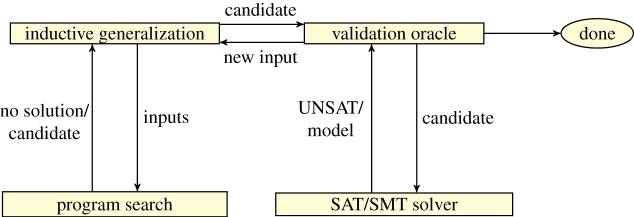
\includegraphics[scale=0.4]{../resources/cegis.jpeg}
        \end{center}
        \caption{CEGIS petlja}
    \end{figure}
\end{frame}

\begin{frame}{CEGIS}
    \begin{itemize}
        \item Da bismo u potpunosti definisali CEGIS sintezu programa, potrebno je odgovoriti na sledeća pitanja:
        \begin{itemize}
            \item Kako treba da izgleda specifikacija traženog programa?
            \item Kako ćemo vršiti sintezu programa kandidata?
            \item Kako da proverimo da li program kandidat zadovoljava specifikacije?
            \item Kako da prosledimo povratne informacije za buduće kandidate?
        \end{itemize}
    \end{itemize}
\end{frame}

\begin{frame}{CEGIS - Sinteza vodjena uzorom}
    \begin{itemize}
        \item \emph{Oracle-guided synthesis}
        \item Pretpostavlja da imamo implementaciju programa koji želimo da sintetišemo - uzor
        \item Uzor se tretira kao crna kutija
        \item Novi test primeri se kreiraju generišući proizvoljne ulaze a od uzora se dobijaju odgovarajući izlazi za svaki prosleđeni ulaz
    \end{itemize}
\end{frame}

\begin{frame}{CEGIS - Stohastička superoptimizacija}
    \begin{itemize}
        \item Pretražuje se prostor programa i traži se brži ili efikasniji ekvivalent polaznog programa
        \item Takođe se pretpostavlja da imamo implementaciju programa kao specifikaciju
        \item Koristi se \emph{MCMC} (eng. \emph{Markov-chain Monte Carlo sampling}) kao mera udaljenosti
    \end{itemize}
\end{frame}

\begin{frame}{CEGIS - Enumerativna pretraga}
    \begin{itemize}
        \item Za specifikaciju se koristi konačan skup test primera
        \item Pretpostavja se da je dostupna gramatika koja opisuje ciljani jezik (\texttt{add(x, sub(x,y))})
        \item Programi se dele prema dubini
        \item Sinteza kreće od dubine $0$ i numerišu se svi programi na toj dubini
        \item Na dubini $k$, ispituju se svi programe koji imaju oblik \texttt{operacija(a,b)}, gde su $a$ i $b$ bilo koji izrazi dubine $k-1$
    \end{itemize}
\end{frame}

\begin{frame}{Zaključak}
    \centering
    \begin{itemize}
        \item Uspešno sintetisanje manjih programa može značajno da olakša rad programerima
        \item Da li će programeri moći da prestanu da govore računarima \textbf{kako} da rade, već da se fokusiraju na to da im kažu \textbf{šta} treba da urade
        \item Najveći potencijal ima induktivna sinteza programa.
        \item CEGIS je, kao vodeći predstavnik ove grupe, u praksi pokazao neočekivano dobre rezultate
    \end{itemize}
\end{frame}

\begin{frame}{Pitanja}
    \centering
    ???
\end{frame}

\begin{frame}{TODO}
    \centering
    Hvala na pažnji!
\end{frame}


\end{document}
